\section{Auswertung}
\label{sec:Auswertung}

\subsection{Wheatston'sche Messbrücke}
Der relative Fehler für $\frac{R_3}{R_4}$ ist mit $0,5\,\%$ und der für $R_2$ ist mit $0,2\,\%$ angegeben. Die Werte für $R_{14}$ und $R_{13}$ sind in
Tabelle \ref{tab:R14} und \ref{tab:R13} zu finden. Mit Hilfe von () lassen sich die Werte
\begin{gather*}
  R_{14} = (704 \pm 631)\,\unit{\ohm} \\
  R_{13} = (1724 \pm 1440)\,\unit{\ohm}
\end{gather*}
bestimmen. Die Fehler aus der Standarabweichung sind wesentlich größer als die angegeben relativen Fehler.

\begin{table}
  \centering
  \caption{Messung von $R_3$ und $R_4$ für $R_{14}$}
  \label{tab:R14}
  \begin{tabular}{c c c c}
    \toprule
    $R_2/\unit{\ohm}$ & $R_3/\unit{\ohm}$ & $R_4/\unit{\ohm}$ & $R_{14}/\unit{\ohm}$ \\
    \midrule
     332 & 243 & 757 &  106,6 \\
     664 & 392 & 608 &  428,1 \\
    1000 & 612 & 388 & 1577,3 \\
    \bottomrule
  \end{tabular}
\end{table}

\begin{table}
  \centering
  \caption{Messung von $R_3$ und $R_4$ für $R_{13}$}
  \label{tab:R13}
  \begin{tabular}{c c c c}
    \toprule
    $R_2/\unit{\ohm}$ & $R_3/\unit{\ohm}$ & $R_4/\unit{\ohm}$ & $R_{13}/\unit{\ohm}$ \\
    \midrule
     332 & 579 & 421 &  456,6 \\
     664 & 595 & 405 &  975,5 \\
    1000 & 789 & 211 & 3739,3 \\
    \bottomrule
  \end{tabular}
\end{table}

\subsection{Kapazitätsmessbrücke}
Der relative Fehler für $R_2$ beträgt $3\,\%$ und der für $C_2$ ist mit $0,2 \,\%$ angegeben. Der relative Fehler des Potentiometers ist gleich geblieben.
$C_2$ ist als $C_2 = 597 \cdot 10^{-9}\,\unit{\farad}$ angegeben. Die Werte für $C_8$ und $R_8$ lassen sich in Tabelle \ref{tab:C8,R8} finden.\\
Mit Hilfe von () und () sind $C_8$ und $R_8$ bestimmt als
\begin{gather*}
  C_8 = (578 \pm 146)\cdot 10^{-9} \,\unit{\farad} \\
  R_8 = (787 \pm 73)\,\unit{\ohm}
\end{gather*}
Auch hier sind die Fehler aus der Standarabweichung wesentlich größer als die angegebenen relativen Fehler.

\begin{table}
  \centering
  \caption{Messung von $C_8$ und $R_8$}
  \label{tab:C8,R8}
  \begin{tabular}{c c c c c}
    \toprule
    $R_2/\unit{\ohm}$ & $R_3/\unit{\ohm}$ & $R_4/\unit{\ohm}$ & $C_8/10^{-9}\unit{\farad}$ & $R_8/\unit{\ohm}$ \\
    \midrule
     500 & 640 & 360 & 336 & 889 \\
     600 & 580 & 420 & 432 & 829 \\
     700 & 480 & 520 & 647 & 646 \\
     800 & 491 & 509 & 619 & 772 \\
     900 & 470 & 530 & 673 & 789 \\
    1000 & 440 & 560 & 760 & 786 \\
    \bottomrule
  \end{tabular}
\end{table}

\subsection{Induktivitätsmessbrücke}


\begin{table}
  \centering
  \caption{Messung von $L_{16}$ und $R_{16}$}
  \label{tab:Cx,Rx}
  \begin{tabular}{c c c c c}
    \toprule
    $R_2/\unit{\ohm}$ & $R_3/\unit{\ohm}$ & $R_4/\unit{\ohm}$ & $L_{16}/10^{-3}\unit{\henry}$ & $R_{16}/\unit{\ohm}$ \\
    \midrule
     500 & 342 & 638 &  268,0 &  7,8 \\
     600 & 430 & 570 &  452,6 & 11,0 \\
     700 & 492 & 508 &  678,0 & 14,1 \\
     800 & 445 & 555 &  641,4 & 11,7 \\
     900 & 527 & 473 & 1002,7 & 16,3 \\
    1000 & 532 & 568 &  936,6 & 13,7 \\
    \bottomrule
  \end{tabular}
\end{table}

\subsection{Maxwellbrücke}

\begin{table}
  \centering
  \caption{Messung von $L_{16}$ und $R_{16}$}
  \label{tab:Cx,Rx,Maxwell}
  \begin{tabular}{c c c c}
    \toprule
    $R_3/\unit{\ohm}$ & $R_4/\unit{\ohm}$ & $L_{16}/10^{-3}\unit{\henry}$ & $R_{16}/\unit{\ohm}$ \\
    \midrule
    222 &  500 &  132,5 & 444 \\
    218 &  600 &  130,1 & 363 \\
    210 &  700 &  125,4 & 300 \\
    175 &  800 &  104,5 & 219 \\
     95 &  900 &   56,7 & 106 \\
      4 & 1000 &    0,2 &   4 \\
    \bottomrule
  \end{tabular}
\end{table}

\subsection{Wien-Robinson-Brücke}
\begin{figure}
  \centering
  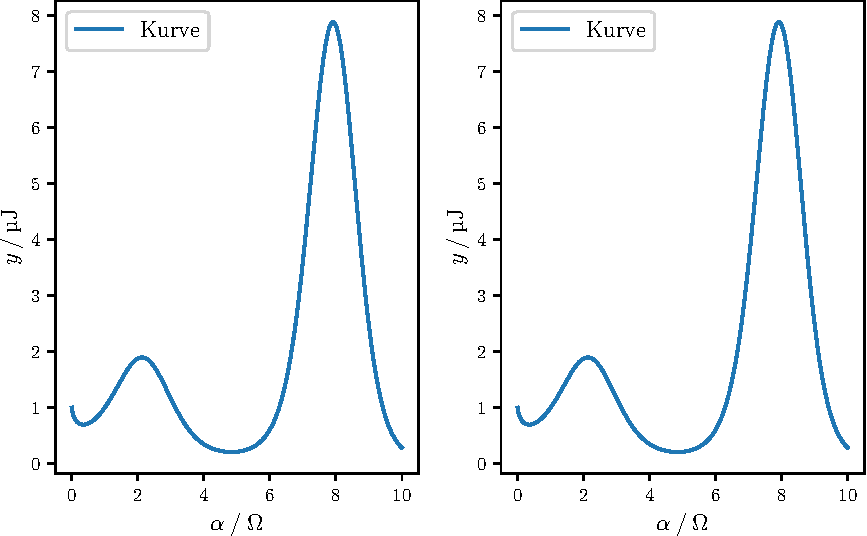
\includegraphics{plot.pdf}
  \caption{Plot.}
  \label{fig:plot}
\end{figure}


Siehe \autoref{fig:plot}!
